\chapter{Background}
\label{chp:background} 

\section{Village Telco}
%How did it all start?

\section{Mesh Potato}
%Generelt om MP

% hvordan MPen fikk navnet. 


%MP01
The whole concept around the Mesh Potato was developed in June 2008 during a workshop at the Shuttleworth Foundation. Including participants like open hardware pioneer Dawid Rowe and Elektra, the developer of the B.A.T.M.A.N. mesh networking protocol \cite{MPworkshop}. The aim was to develop a business model as well as a prototype for a Village Telco. Initially the idea was to use low cost VoIP headsets. At that time it was the most viable and convenient way to deliver telephone services to the customers. With a VoIP telephone services the nodes can not be more than 100 meters away from each other, requiring more nodes in order to cover the desirable area. Which again would drastically increase the start-up costs for a village. In order to keep the cost down, it was also important to keep the number of access points down. A mesh network have a larger range, and one suggestion was to use a small mesh device like a Open Mesh AP and connect a SIP phone to it. This solution would solve a lot of the problems regarding range, antenna and number of access points, but the idea was still an expensive option. The challenge was to create something that would be simple enough to be implemented and scaled by local entrepreneurs with limited technical skills. 
During the debating, Rael Lissoos took a Analogue Telephone Adapter (ATA) and an Open Mesh AP, held them together and said that we need these two devices in one. This point was the birth of the Mesh Potato. The name comes from combining the words mesh, POTS (Plain Old Telephone) and ATA. "Patata" is the Spanish word for potato, and hence the name Mesh Potato. A mesh enabled WiFi device with the possibility to connect any inexpensive regular phone and IP device. \cite{MPorigin}

\begin{figure}[h!]
  \centering
      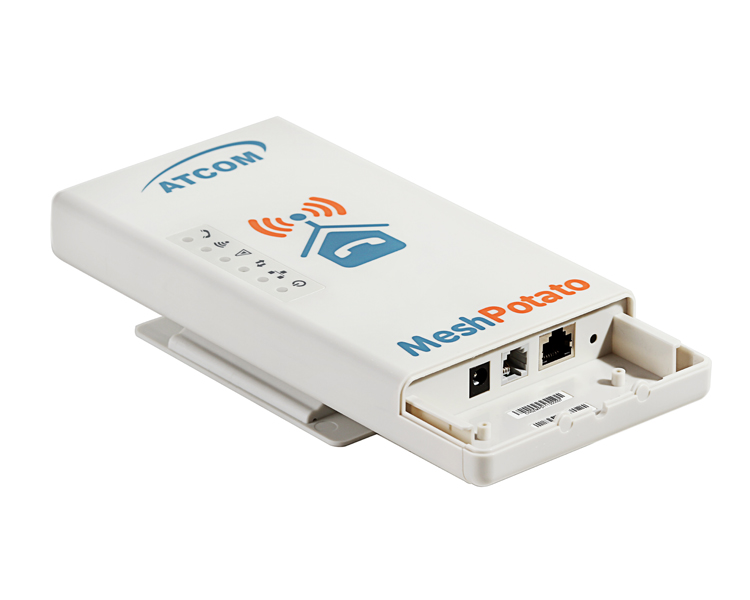
\includegraphics[width=0.5\textwidth]{MP01}
  \caption [The Mesh Potato]{\textbf{The fist generation Mesh Potato, MP01}}
  \label{fig:MP01}
\end{figure}

The First generation of the Mesh Potato is shown in \fref{fig:MP01}. This device is designed to be used in rural areas. It can be deployed and run anywhere in the world relying only on a low, but stable, power supply. The Ethernet port, Foreign eXchange Station (FXS) ports and power are robust and designed in order to handle hard weather, poor power conditions, lightening and static electricity. In addition the Mesh Potato comes in a waterproof box for outdoor mounting \cite{background}.

The Mesh Potato combines the features of a 802.11bg WiFi router with an Analog telephone Adaptor (ATA) \cite{MP}. Each Mesh Potato provides a single fixed telephone line to the end user. The MPs are connected together via a mesh WiFi network, and  configure themselves automatically to form a peer-to-peer network, greatly extending the range of the network over regular WiFi. Enabling phone calls to be made independent of landlines and telephone towers. Creating the basis for the "plug-and-play" solution. 

The device is based on the Atheros chipset that if used, among others, by OpenMesh, and woould run OpenWRT and B.A.T.M.A.N.







The Mesh network can be connected via backbone link to the rest of the world by using VoIP trunks. 


MP02





\section{Technology}

\subsection{Ad Hoc and Mesh Networks}

\begin{figure}[h!]
  \centering
    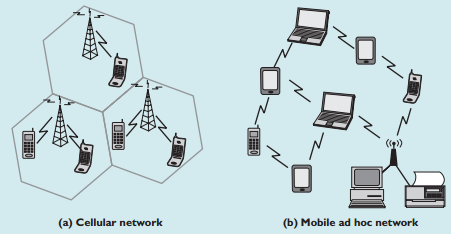
\includegraphics[width=0.8\textwidth]{adhoc.png}
     \caption [Cellular network vs. MANET]{\textbf{Cellular network vs. MANET}. This figure illustrates the difference between a regular cellular network and a mobile ad hoc network \cite{adhoc2}.}
\label{fig:adhoc}
\end{figure}

\subsubsection{MANETs} Mobile ad hoc networks (MANETs) are networks that does not rely on an underlying and fixed infrastructure (access points and routers), in other words infrastructureless. MANETs acts in a shared wireless media \cite{adhoc}. The structure of these networks change dynamically, and key factors for MANETs is self-configuration and self-organization. The members of the network are mobile and are free to join or leave the network \cite{adhoc2}, and therefore these factors are important. MANETs are based on multi-hop forwarding. This means that each node acts not only as a host, but also as a router. The nodes themselves establishes and maintain routes, and forward packets to other nodes if necessary. This enables communication between nodes that are originally not within each other's send range \cite{adhoc2}. Because of these characteristics MANETs is suited for use in situations where there are no fixed underlying infrastructure. MANETs can operate as a stand-alone solution, but it can also be attached to the Internet. This makes room for numerous of services. 

\begin{figure}[h!]
  \centering
    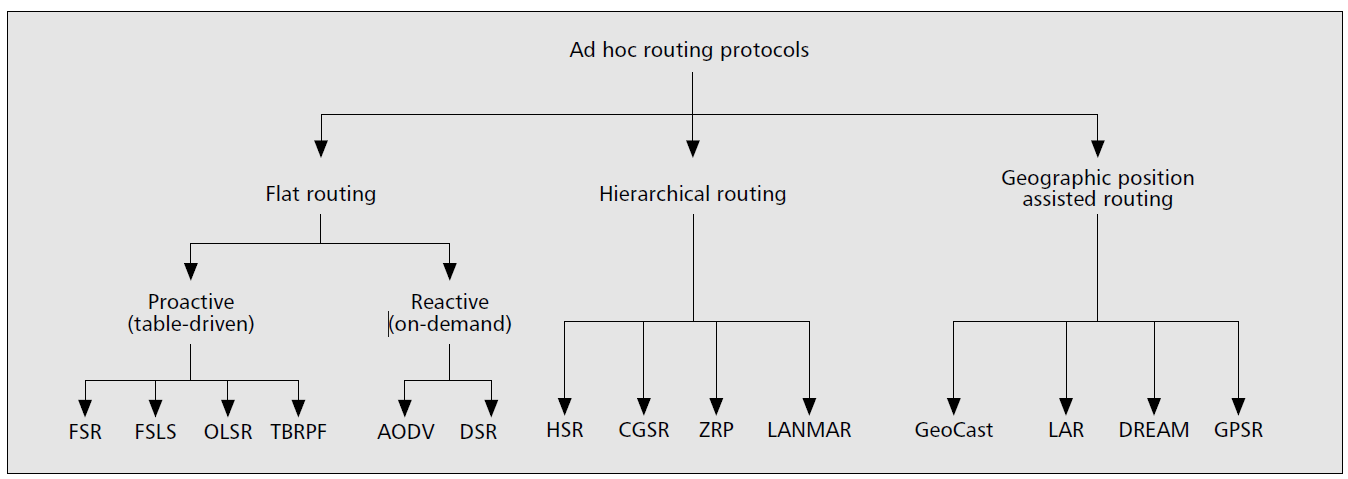
\includegraphics[width=1\textwidth]{adhocprotocols.png}
     \caption{Different groups of ad hoc routing protocols \cite{adhoc}.}
\label{fig:adhocprotocols}
\end{figure}


\subsubsection{Routing Protocols}
There exists many challenges when it comes to these types of networks. The routing protocols must be able to adapt quickly due to the topology changes. \fref{fig:adhocprotocols} shows the different groups of the ad hoc protocols that exist. The routing protocols must not cause excessive overhead. Under the category flat routing, there are two types of routing protocols; proactive and reactive. \textit{Proactive routing protocols} (e.g. OLSR) are table driven \citep{proactivereactive}. This means that every network node has a routing table for the forwarding of data. To obtain stability, each node broadcasts and modifies the routing table periodically. Proactive routing protocols are suitable when there are few nodes in the network. Because of the routing table that is periodically updated, the overhead exceeds the desired value when there are a high number of nodes in the network. In contrary to the proactive routing protocols, \textit{reactive routing protocols} (e.g. AODV) are on demand. Since they are on demand, the overhead is significantly lower. These protocols utilizes flooding. The network is flooded with the route request (RREQ) in order to set up the route. The reactive routing protocols does not have a up-to-date routing table like proactive routing protocols \cite{proactivereactive}. Routes are only set up to nodes they communicate with, and these routes are only kept alive while they are needed  \cite{adhoc2}. As shown in \fref{fig:adhocprotocols}, there are several different protocols under proactive and reactive. 

\paragraph{B.A.T.M.A.N}
Better Approach To Mobile Adhoc Networking (B.A.T.M.A.N) is the routing protocol utilized in the networks formed by the Mesh Potatoes. B.A.T.M.A.N is a proactive routing protocol for wireless ad hoc networks. This includes MANETs \cite{batman}. This protocol was developed as an alternative to OLSR (Optimized Link State Routing) \cite{batman2}. Like mentioned before, routing protocols must be able to adapt quickly to topology changes. B.A.T.M.A.N was made to be a more efficient routing protocol in this area, since it employs a new method for discovering routes. The nodes in the network broadcasts a OGM periodically. A OGM is a Originator Message which contains: 

\begin{itemize}
\item The address of the node
\item Sequence number
\item TTL (Time to live)
\end{itemize}

The address and the sequence number enables identification of a packet and duplicate detection. 

\begin{figure}[h!]
  \centering
    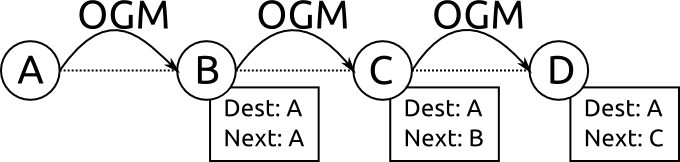
\includegraphics[width=0.8\textwidth]{batman.png}
     \caption{SKRIVE NOE HER \cite{batman2}.}
\label{fig:batman} 
\end{figure}


Information about the nodes that are accessible via single-hop or multi-hop are maintained and updated \cite{batman}. Every node updates it's routing table each time it receives and OGM. The routing table includes information about \cite{batman2}:

\begin{description}
  \item[Originator Address] \hfill \\
  This is the source address of the node that sent the OGM.
  \item[Current Sequence Number] \hfill \\
  The sequence number of the last OGM. This is used to discover if there are any duplicates or any information that is outdated.
  \item[Sliding Window] \hfill \\
  A list of sequence numbers that is stored for each originator and each previous hop, i.e., for the neighbour node that forwarded or originated the OGM. 
 
  
%The sliding windows are used to determine the best next hop for each destination
\end{description}

When a node receives an OGM it will decrease the TTL, and then forward it to the neighbour nodes. The same OGM can arrive to a node, but from a different paths. In this case, only the first copy is preserved. 

%Eksempel på nettverk

\subsection{OpenWrt}

\section{The Cost Structure and Revenue Model(s) of Village Telco Today}

\section{Comparison of Village Telco and Other Telcos}

\section{Refugee Camps}
\subsection{The Existing Communication Methods}